\appendix
\section{Tracciamento dei requisiti}
\label{sec:Tracciamento}

\normalsize
\begin{longtable}{|c|c|}
	\hline
	\textbf{Codice Requisiti} & \textbf{Implementazione} \\
	\hline
	\endhead
	R0F1 & Implementato\\
	\hline
	R0F1.1  & Implementato\\
	\hline
	R0F1.1.1  & Implementato\\
	\hline
	R0F1.1.2  & Implementato\\
	\hline
	R0F1.1.3 & Non implementato\\
	\hline
	R1F1.2.1 & Implementato\\
	\hline
	R1F1.2.2 & Implementato\\
	\hline
	R1F1.2.3 & Non implementato\\
	\hline
	R1F1.3 & Implementato\\
	\hline
	R2F1.3.1 & Non implementato\\
	\hline
	R1F1.3.2 & Implementato\\
	\hline
	R1F1.4 & Implementato\\
	\hline
	R2F1.4.1 & Implementato\\
	\hline
	R2F1.4.2 & Non implementato\\
	\hline
	R0F1.5 & Implementato\\
	\hline
	R2F1.5.1 & Implementato\\
	\hline
	R2F1.5.1.1 & Non implementato\\
	\hline
	R2F1.5.1.2 & Implementato\\
	\hline
	R0F1.5.2 & Implementato\\
	\hline
	R0F1.5.2.1 & Implementato\\
	\hline
	R0F1.5.2.2 & Implementato\\
	\hline
	R1F1.6 & Implementato\\
	\hline
	R1F1.6.1 & Implementato\\
	\hline
	R1F1.6.2 & Implementato\\
	\hline
	R1F1.6.2.1 & Implementato\\
	\hline
	R1F1.6.2.2 & Non implementato\\
	\hline
	R2F1.7 & Implementato\\
	\hline
	R2F1.7.1 & Implementato\\
	\hline
	R2F1.7.2 & Implementato\\
	\hline
	R2F1.7.3 & Non implementato\\
	\hline
	R1F1.8 & Non implementato\\
	\hline
	R0F2 & Implementato\\
	\hline
	R0F2.1 & Implementato\\
	\hline
	R1F2.1.1 & Implementato\\
	\hline
	R0F2.1.2 & Implementato\\
	\hline
	R1F2.1.3 & Implementato\\
	\hline
	R1F2.1.4 & Implementato\\
	\hline
	R0F2.1.5 & Implementato\\
	\hline
	R1F2.1.5.1 & Non implementato\\
	\hline
	R1F2.2 & Non implementato\\
	\hline
	R1F2.2.1 & Non implementato\\
	\hline
	R1F2.2.1.1 & Non implementato\\
	\hline
	R1F2.2.1.2 & Non implementato\\
	\hline
	R1F2.2.2 & Non implementato\\
	\hline
	R1F2.2.2.1 & Non implementato\\
	\hline
	R1F2.2.2.2 & Non implementato\\
	\hline
	R1F2.4 & Non implementato\\
	\hline
	R0F3 & Implementato\\
	\hline
	R0F3.1 & Implementato\\
	\hline
	R0F3.1.1 & Implementato\\
	\hline
	R1F3.1.2 & Implementato\\
	\hline
	R1F3.1.3 & Implementato\\
	\hline
	R2F3.1.4 & Implementato\\
	\hline
	R2F3.2 & Implementato\\
	\hline
	R2F3.2.1 & Implementato\\
	\hline
	R2F3.2.2 & Implementato\\
	\hline
	R1F4 & Implementato\\
	\hline
	R1F4.1 & Implementato\\
	\hline
	R1F4.1.1 & Implementato\\
	\hline
	R1F4.1.2 & Implementato\\
	\hline
	R1F4.1.3 & Implementato\\
	\hline
	R1F4.1.4 & Implementato\\
	\hline
	R1F4.1.5 & Implementato\\
	\hline
	R1F4.2 & Non implementato\\
	\hline
	R1F4.2.1 & Non implementato\\
	\hline
	R1F4.2.1.1 & Non implementato\\
	\hline
	R1F4.2.1.2 & Non implementato\\
	\hline
	R1F4.2.2 & Non implementato\\
	\hline
	R1F4.2.2.1 & Non implementato\\
	\hline
	R1F4.2.2.2 & Non implementato\\
	\hline
	\caption[Tracciamento Requisiti Funzionali]{Tracciamento Requisiti Funzionali}
\end{longtable}

\section{Resoconto delle attività di verifica}
	\subsection{Riassunto delle attività di verifica}
	\subsubsection{Revisione dei requisiti}
	L'attività di verifica, compito del \emph{\gl{Verificatore}}, è stata effettuata in corrispondenza della terminazione della stesura di ogni documento. La verifica dei documenti è stata eseguita facendo riferimento alle indicazioni contenute nelle \emph{Norme di Progetto v1.0.0} e misurando le metriche specificate in questo documento.
	\subsubsection{Revisione di progettazione}
	L'attività di verifica, compito del \emph{Verificatore}, è stata effettuata successivamente all'incremento di ogni documento. La verifica è stata eseguita facendo riferimento alle indicazioni contenute nelle \emph{Norme di Progetto v2.0.0} e misurando le metriche specificate in questo documento.
	\subsubsection{Revisione di qualifica}
	L'attività di verifica, compito  del \emph{Verificatore}, è stata effettuata successivamente all'incremento di ogni documento.
	Diversamente dalle precedenti consegne in questa fase le misurazioni sono state effettuate più volte per ogni metrica definita nel documento \emph{Norme di Progetto v3.0.0}, così facendo abbiamo ottenuto dei grafici utili a comprendere la qualità del progetto durante il suo sviluppo.
	
	\subsection{Dettaglio delle verifiche tramite analisi}
	\subsubsection{Misurazioni}
	\paragraph{Rischi non individuati} \Spazio
	nonostante qualche ritardo nella stesura della \textit{Product Baseline} il gruppo è riuscito a recuperare e a consegnare tutti i documenti nei tempi previsti. 
	\begin{figure}[H]
		\centering 
		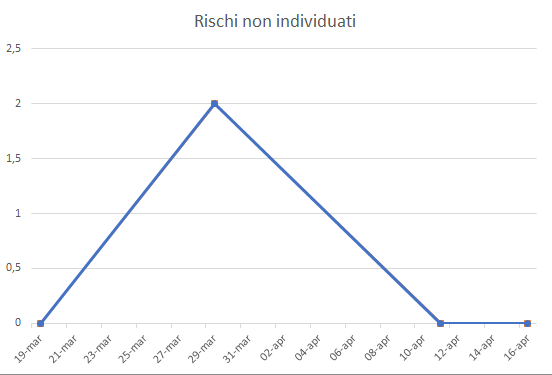
\includegraphics[width=0.7\textwidth]{Images/rischiNI.png}
		\caption{Serie storica dei rischi non individuati}
		\label{rischi} 
	\end{figure}
    \paragraph{Requisiti obbligatori soddisfatti} \Spazio
    Il gruppo in entrata alla \emph{Revisione di Qualifica} è riuscito a soddisfare quasi tutti i requisiti obbligatori previsti dal documento \textit{Analisi dei Requisiti v 2.0.0}.
    \begin{figure}[H]
    	\centering 
    	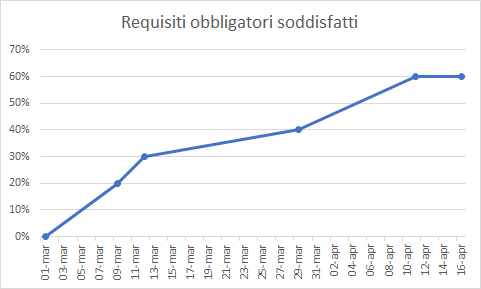
\includegraphics[width=0.7\textwidth]{Images/obbl.png}
    	\caption{Serie storica dei requisiti obbligatori soddisfatti}
    	\label{obbl} 
    \end{figure}
    \paragraph{Structural fan-in} \Spazio
    Questo indice va massimizzato, visto però il numero limitato di componenti è difficile ottenere un valore alto.
    \begin{figure}[H]
    	\centering 
    	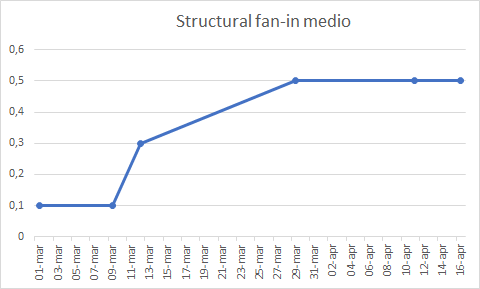
\includegraphics[width=0.7\textwidth]{Images/SFIN.png}
    	\caption{Serie storica del Structural fan-in}
    	\label{SFIN} 
    \end{figure}
    \paragraph{Structural fan-out} \Spazio
    Questo indice va minimizzato, il gruppo è sempre riuscito a mantenere il suo valore nel range ottimale.
    \begin{figure}[H]
    	\centering 
    	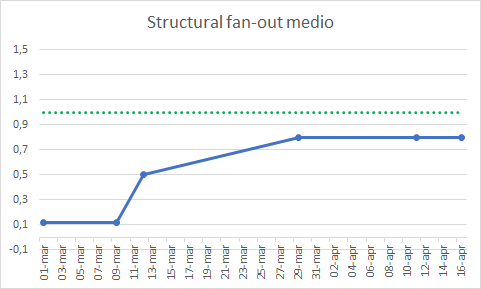
\includegraphics[width=0.7\textwidth]{Images/SFOUT.png}
    	\caption{Serie storica del Structural fan-out}
    	\label{SFOUT} 
    \end{figure}
    \paragraph{Metodi per classe} \Spazio
    il gruppo è sempre riuscito a mantenere questo valore nel range ottimale grazie alla progettazione di classi non troppo complesse.
    \begin{figure}[H]
    	\centering 
    	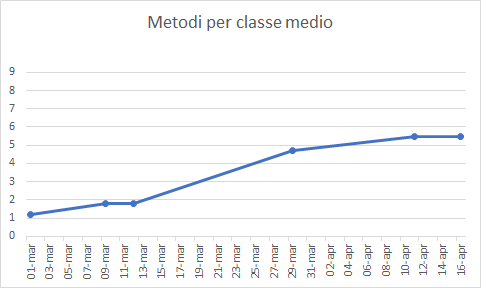
\includegraphics[width=0.7\textwidth]{Images/metodi.png}
    	\caption{Serie storica dei metodi per classe medio}
    	\label{metodi} 
    \end{figure}
    \paragraph{Parametri per metodo} \Spazio
    I metodi che sono stati creati non superano i tre parametri perciò il risultato medio è sempre stato nel range ottimale.
    \begin{figure}[H]
    	\centering 
    	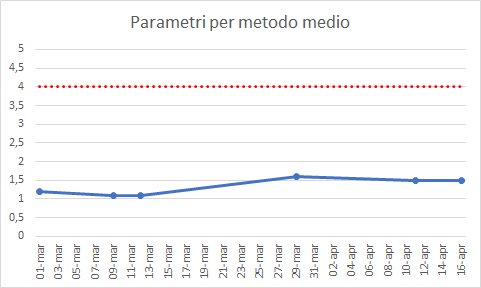
\includegraphics[width=0.7\textwidth]{Images/parametri.png}
    	\caption{Serie storica dei parametri per metodo medio}
    	\label{parametri} 
    \end{figure}
    \paragraph{Complessità ciclomatica} \Spazio
    Dopo una iniziale fuoriuscita dal range di accettazione dovuto alla scarsa conoscenza di Kibana il gruppo è riuscito a riportare questo valore nel range ottimale.
    \begin{figure}[H]
    	\centering 
    	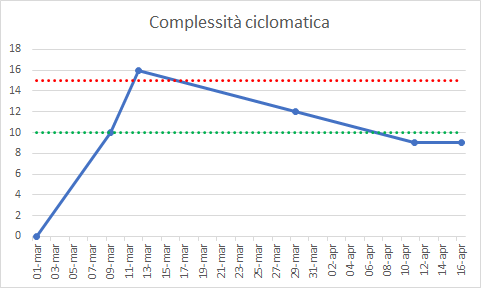
\includegraphics[width=0.7\textwidth]{Images/ciclo.png}
    	\caption{Serie storica della complessità ciclomatica media}
    	\label{ciclo} 
    \end{figure}
    \paragraph{Linee di codice per linee di commento} \Spazio
    Dopo una iniziale carenza di linee di commento il gruppo si è impegnato per portare questo valore in un range accettabile.
    \begin{figure}[H]
    	\centering 
    	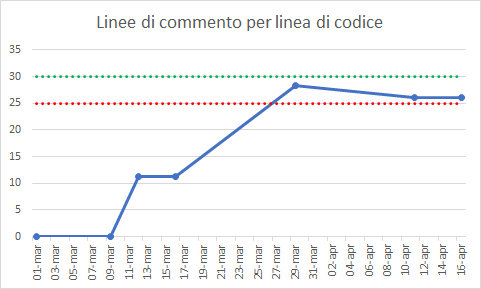
\includegraphics[width=0.7\textwidth]{Images/comm.png}
    	\caption{Serie storica delle linee di codice per linee di commento}
    	\label{comm} 
    \end{figure}
    \paragraph{Indice di gulpease} \Spazio
    Il gruppo è sempre riuscito a mantenere questo indice all'interno del range ottimale.
    \begin{figure}[H]
    	\centering 
    	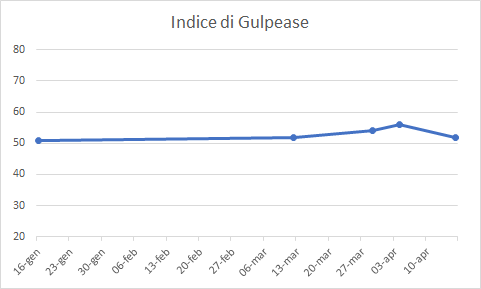
\includegraphics[width=0.7\textwidth]{Images/Gulpease.png}
    	\caption{Serie storica dell'indice di gulpease medio}
    	\label{gul} 
    \end{figure}
    \paragraph{Branch coverage} \Spazio
    I test dinamici in questo momento percorrono la maggior parte dei rami decisionali presenti. 
    \begin{figure}[H]
    	\centering 
    	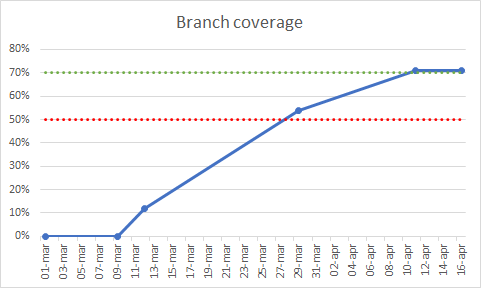
\includegraphics[width=0.7\textwidth]{Images/branch.png}
    	\caption{Serie storica del branch coverage}
    	\label{branch} 
    \end{figure}
    \paragraph{Statement coverage} \Spazio
    La maggior parte del codice viene eseguito dai test dinamici presenti.
    \begin{figure}[H]
    	\centering 
    	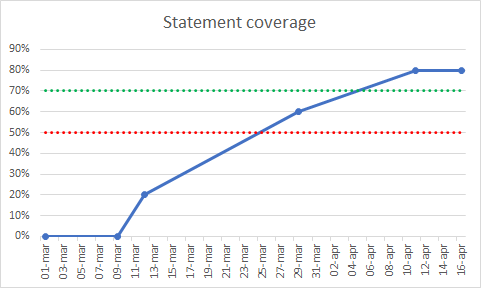
\includegraphics[width=0.7\textwidth]{Images/statement.png}
    	\caption{Serie storica dello statement coverage}
    	\label{statement} 
    \end{figure}
    \paragraph{Completezza dell'implementazione funzionale} \Spazio
    Il gruppo ha raggiunto una buona copertura dei requisiti funzionali già in entrata alla \emph{Revisione di Qualifica}.
    \begin{figure}[H]
    	\centering 
    	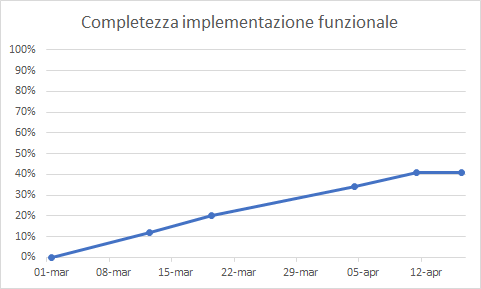
\includegraphics[width=0.7\textwidth]{Images/completezza-funzionale.png}
    	\caption{Serie storica della completezza dell'implementazione funzionale}
    	\label{cf} 
    \end{figure}
     \paragraph{Densità di failure} \Spazio
    Inizialmente la percentuale di test falliti era abbastanza alta ma il gruppo è riuscito a portare questo valore in un range accettabile.
    \begin{figure}[H]
    	\centering 
    	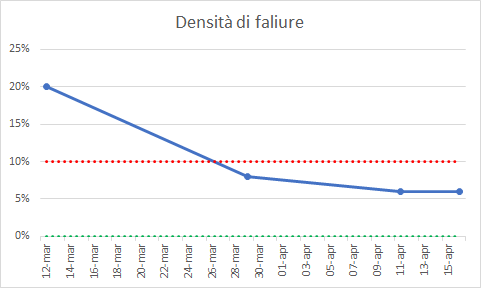
\includegraphics[width=0.7\textwidth]{Images/fail.png}
    	\caption{Serie storica della densità di failure}
    	\label{fail} 
    \end{figure} 
    \paragraph{Comprensibilità delle funzionalità offerte} \Spazio
    Questo valore è quasi sempre rimasto in un range ottimale visto che il nostro prodotto è di natura semplice e intuitivo.
    \begin{figure}[H]
    	\centering 
    	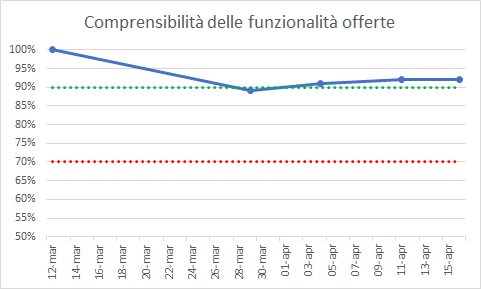
\includegraphics[width=0.7\textwidth]{Images/compr.png}
    	\caption{Serie storica della Comprensibilità delle funzionalità offerte}
    	\label{compr} 
    \end{figure}
    \paragraph{Facilità di apprendimento} \Spazio
    Questo valore è aumentato con l'aumentare della complessità del prodotto ma è sempre rimasto sempre nel range ottimale.
    \begin{figure}[H]
    	\centering 
    	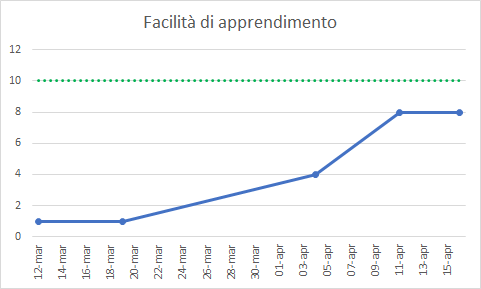
\includegraphics[width=0.7\textwidth]{Images/fac.png}
    	\caption{Serie storica della facilità di apprendimento}
    	\label{fac} 
    \end{figure}
    \paragraph{Tempo di risposta} \Spazio
    Il tempo di risposta non è mai fuoriuscito dal range ottimale ma potrebbe nel caso in cui la connessione utilizzata sia lenta.
    \begin{figure}[H]
    	\centering 
    	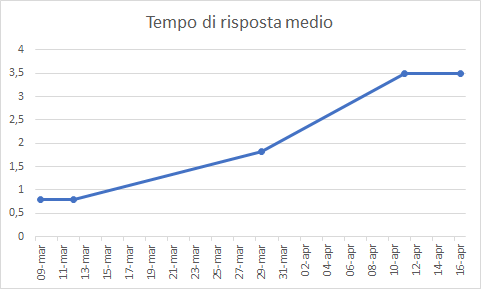
\includegraphics[width=0.7\textwidth]{Images/risposta.png}
    	\caption{Serie storica del tempo di risposta medio}
    	\label{risposta} 
    \end{figure}
    \paragraph{Capacità di analisi failure} \Spazio
    Il gruppo è stato in grado di trovare la maggior parte degli errori che portavano al fallimento di un test.
    \begin{figure}[H]
    	\centering 
    	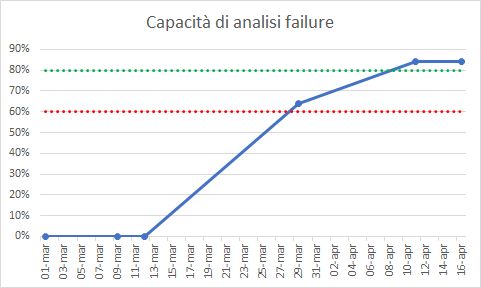
\includegraphics[width=0.7\textwidth]{Images/cap.png}
    	\caption{Serie storica della capacità di analisi failure}
    	\label{cap} 
    \end{figure}
     \subparagraph{Impatto delle modifiche} \Spazio
    All'aumentare della complessità del codice questo valore è aumentato ma è sempre rimasto in un range accettabile.
    \begin{figure}[H]
    	\centering 
    	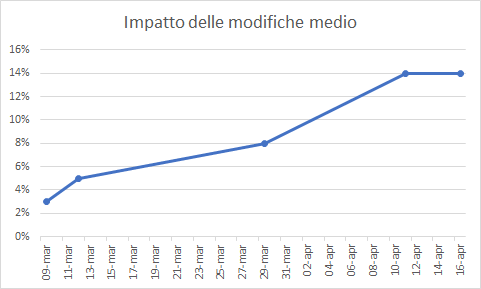
\includegraphics[width=0.7\textwidth]{Images/modifiche.png}
    	\caption{Serie storica dell'impatto delle modifiche}
    	\label{modifiche} 
    \end{figure}
